\documentclass[]{article}
\usepackage{amsmath,amssymb}
\usepackage{lmodern}
\usepackage{iftex}
\usepackage{ragged2e}
\usepackage{stackengine}
\usepackage{dirtytalk}
\usepackage{graphicx}
% \graphicspath{{./images/}}


\hbadness=99999

\date{\today}
\author{ID: 14221}
\title{Submission 2.1}

\begin{document}

\maketitle

\begin{enumerate}
    % \setcounter{enumi}{1}
    \item Translate into smooth English:
    \begin{center}
        $\forall x \forall y((Px \land Ty \land Dxy \land Oxy)\Rightarrow \neg \exists z(Pz \land Kzxy)).$
    \end{center}
    Let \say{Px} mean \say{x is a person}, and \say{Tx} mean \say{x is a time}, and \say{Dxy} mean \say{x is down at time y}, and \say{Oxy} mean \say{x is out at time y}, and \say{Kxyz} mean \say{x knows y at time z}.
    \\\\ For all x and all y, if x is a person, and y is a time, x is down at time y, and x is out at time y then there doesn't exist a person z that knows x at time y.
    
    
    \item 2. All’s well that ends well. (Shakespeare)
    \newline W: It is well
    \newline E: Ends well
    \newline $\forall x (Ex \Rightarrow Wx)$
    
    
    

    \item ...the things which are seen are temporal; but the things which are not seen are eternal. (II Corinthians 4:18)
    \newline S: Things are seen
    \newline T: Things are temporal
    \newline E: Things are eternal
    % \newline $T \land \neg E$
    \\\\ $\forall x (Sx \Rightarrow Tx) \land (\neg Sx \Rightarrow Ex)$
    
    \item  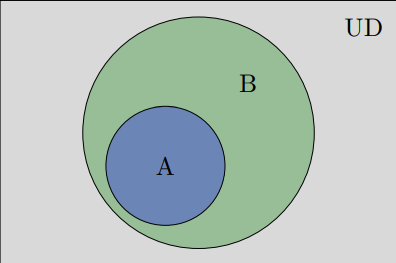
\includegraphics[scale=0.5]{Sub2.1Q4.png}
    \newline $\forall x(Ax \Rightarrow Bx)$
    
    \item 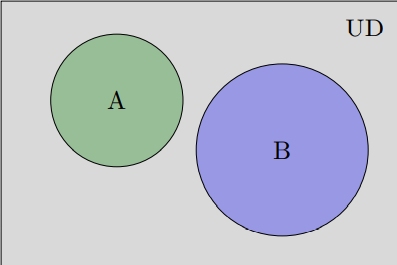
\includegraphics[scale=0.5]{Sub2.1Q5.png}
    \newline $\forall x(Ax \Rightarrow \neg Bx)$
    
    \item If you don’t love yourself, you can’t love anybody else
    \newline y: yourself
    \newline Lxy: x loves y
    \newline x: All people
    \\\\ $\forall x \forall y(\neg Lyy \Rightarrow \neg Lyx)$
    
    \item N Sync is the best band ever.
    \newline n: N Sync
    \newline x: All bands
    \newline Bnx: n is the best band of x
    \newline $\forall x (Bnx)$
    
    \item  Somebody loves everybody.
    \newline s: Somebody
    \newline x: everybody
    \newline Lxy: x loves y
    \newline $\exists s \forall x  (Lsx)$
    
    \item There is someone for everybody.
    \newline s: Someone
    \newline e: Everybody
    \newline Txy: x is there for y
    \newline $\exists s \forall e  (Tse)$
    
    \item Scrooge doesn’t love anybody.
    \newline s: Scrooge
    \newline e: Everybody
    \newline Lxy: x loves y
    \newline $\forall e (\neg Lse)$

    
    \item Only the shallow know themselves. (Oscar Wilde)
    \newline s: shallow people
    \newline t: themselves
    \newline Kxy: Only x know y
    \newline $\exists s (Kst)$
    
    \item Everybody has a mother.
    \newline m: mother
    \newline Hxy: x has a y
    \newline $\forall x \exists m (Hxm)$
    
    \item  There are at least two pigs.
    \newline Px: x is a pig
    \newline $\exists x \exists y (\neg x = y \land P(x)\land P(y))$
    
    \item There are exactly two pigs.
    \newline Px: x is a pig
    \newline $\exists x \exists y((\neg x = y)\land (Px \land Py))\land\forall z (Pz \Rightarrow (x = z \lor y=z))$

    \item There are at most two pigs.
    \newline Px: x is a pig
    \newline $\forall x \forall y \forall z(Px \land Py \land Pz) \Rightarrow (x=y \lor x=z \lor y=z)$
    
\end{enumerate}




\end{document}
